%!
%! Copyright (C) 2015 - Present Andrea Dal Corso 
%! This file is distributed under the terms of the
%! GNU General Public License. See the file `License'
%! in the root directory of the present distribution,
%! or http://www.gnu.org/copyleft/gpl.txt .
%!
\documentclass[12pt,a4paper]{article}
\def\version{1.1.0}
\def\qe{{\sc Quantum ESPRESSO}}
\def\tpw{{\sc THERMO\_PW}}
\def\thermo{{\texttt{thermo\_pw}}}

\usepackage{html}
\usepackage{color}

\usepackage{graphicx}

\definecolor{web-blue}{rgb}{0,0.5,1.0}
\definecolor{coral}{rgb}{1.0,0.5,0.3}
\definecolor{red}{rgb}{1.0,0,0.0}
\definecolor{green}{rgb}{0.,1.0,0.0}

\textwidth = 17cm
\textheight = 24cm
\topmargin =-1 cm
\oddsidemargin = 0 cm

\def\pwx{\texttt{pw.x}}
\def\phx{\texttt{ph.x}}
\def\configure{\texttt{configure}}
\def\PWscf{\texttt{PWscf}}
\def\PHonon{\texttt{PHonon}}
\def\make{\texttt{make}}

\begin{document}
\author{Andrea Dal Corso (SISSA - Trieste)}
\date{}

%\def\SissaImage{./sissa_on_white.png}

\title{
%  \includegraphics[width=6cm]{\SissaImage}\\
  \vskip 1cm
  {\color{red}\Huge \tpw\ Developer's Guide} \\
  \Large (version \version)
}
\maketitle

\tableofcontents

\newpage

\section{\color{coral}Introduction}
This guide discusses the internal organization of \tpw. It is not necessary
to read it to use \tpw. It contains some technical information not 
appropriate for the user's guide that you might need to modify the code.
It assumes that you have read and understood the user's guide and that
you have already some familiarity with the input variables and 
the working modes of \tpw.

\section{\color{coral}People}
This guide has been written by Andrea Dal Corso (SISSA - Trieste). 

\newpage
\section{\color{coral}Overview}
\tpw\ is logically divided into parts. In some parts the different
images run asynchronously doing different tasks and in some parts the
run is synchronous. Usually in this synchronous parts results are 
collected, the image division of the processors is not used, and when possible
the work is parallelized among all available processors. In some cases
only the processors of the root image make the work while the others remain
idle.
Presently \tpw\ has two asynchronous runs each one followed
by one or more synchronous parts. The parts that are activated in
each run depend on the input variable \texttt{what}. After reading the input,
and writing some summary, the code calls the routine 
\texttt{initialize\_thermo\_work} that sets all the
logical flags that control the global run and the first asynchronous
part. The first asynchronous part (A) makes \texttt{nwork} \texttt{pw.x} 
calculations in parallel in each image. 
Then the following synchronous part makes one or more of
the following calculations:
\begin{itemize}

\item
B) \texttt{lconv\_ke\_test=.TRUE.} writes and plots the total
energy as a function of the kinetic energy.

\item
C) \texttt{lconv\_nk\_test=.TRUE.} writes and plots the total energy
as a function of the {\bf k}-points set.

\item
D) \texttt{lev\_syn\_1=.TRUE.} makes a Murnaghan fit of the 
total energy/enthalpy as a function of the unit cell volume or 
a quadratic/quartic fit of the total energy / enthalpy as a function 
of the crystal parameters and determines the minimum energy geometry.

\item
E) \texttt{lpwscf\_syn\_1=.TRUE.} makes a self-consistent \texttt{pw.x} 
calculation.

\item
F) \texttt{lband\_syn\_1=.TRUE.} makes a non self-consistent \texttt{pw.x}
calculation to compute the band structure.

\end{itemize}

The second part can have an asynchronous part in which
many \texttt{pw.x} calculations are made (\texttt{lpart2\_pw=.TRUE.}) (G1)
or a loop of asynchronous phonon runs (G2), one for each geometry calculated
in A or at the minimum energy/enthalpy geometry
found in D whose self-consistent calculation has been done in E.
The G2 run is controlled by \texttt{lph=.TRUE.}, by \texttt{tot\_ngeo} which 
is the number of geometries, and by the flag 
\texttt{all\_geometries\_together}. When the latter is .FALSE.,
for each geometry the code calculates the phonon dispersions, the phonon 
dos and the 
harmonic thermodynamic quantities. The geometry to do is controlled only 
changing the \texttt{outdir} directory where the phonon run finds the
files produced by the \texttt{pw.x} calculation. The final collection
of the dynamical matrices, calculations of the phonon dispersions, phonon 
dos and harmonic thermodynamic quantities are done in a synchronous way 
within the loop over the geometries.
When \texttt{all\_geometries\_together=.TRUE.} a single asynchronous run
calculates all the irreducible representations of all geometries. After
the phonon run, the phonon dispersions, phonon dos and harmonic 
thermodynamic quantities are calculated synchronously in a loop over 
the geometries.

Following G1 or G2 there is another synchronous part. 
After G1 the synchronous part will do one of the following:

\begin{itemize}

\item
H) \texttt{lelastic\_const=.TRUE.} elastic constants calculations.

\item
I) \texttt{lpiezoelectric\_tensor=.TRUE.} piezoelectric tensor calculation.

\item
L) \texttt{lpolarization=.TRUE.} polarization calculation.

\end{itemize}

After G2, depending on \texttt{what} the synchronous part will do nothing, 
or if the phonons have been computed for several geometries it will do:

\begin{itemize}

\item
M) the interpolation and minimization of the 
Helmholtz or Gibbs free energy at any temperature.

\item
N) Calculation of the Gr\"uneisen parameters on a path over the Brillouin
zone and their plot.

\item
O) Calculation of the anharmonic quantities such as the thermal expansion
from the numerical differentiation of the crystal parameters. Calculation
of the isoentropic quantities when available.

\item
P) Calculation of the Gr\"uneisen parameters on a uniform mesh of {\bf q} 
points and calculation of the thermal expansion from the Gr\"uneisen parameters.
Calculation of the isoentropic quantities when available.

\end{itemize}
There is also an initial routine (\texttt{thermo\_summary}) that can carry
out preprocessing tasks, such as finding the space group or suggesting
alternative \texttt{ibrav} and \texttt{celldm}. This routine is called by
all \texttt{what} options.

\newpage
\section{\color{coral}Activated parts}

The different \texttt{what} activates the following parts of the code:

\begin{verbatim}
what         A   B   C   D   E    F     G1    H    I   L   G2   M   N   O   P

plot_bz
scf                          *
scf_ke       *   *
scf_nk       *       *
scf_bands                    *    *
scf_2d_bands                 *    *
scf_dos                      *    *
scf_ph                       *                              *
scf_disp                     *                              *
scf_elastic_constants                    *     *
scf_piezoelectric_tensor                 *          +
scf_polarization                         *              +
mur_lc       *           *
mur_lc_bands *           *   *    *
mur_lc_dos   *           *   *    *
mur_lc_ph    *           *   *                              *
mur_lc_disp  *           *   *                              *
mur_lc_elastic_constants
             *           *               *      *
mur_lc_piezoelectric_tensor
             *           *               *          +
mur_lc_polarization
             *           *               *               +
mur_lc_t     *           *                                   *     *  *   *  *
elastic_constants_t                      *      *  

+ not yet active or working.
\end{verbatim}

\newpage

\section{\color{coral}Plots and physical quantities}
This is the list of the plots that can be obtained and 
the \texttt{what} to use:

\begin{verbatim}
Brillouin zone                                 plot_bz
X-ray powder diffraction pattern               plot_bz
Total energy versus kinetic energy             scf_ke
Total energy versus k points                   scf_nk
Total energy as a function of volume           mur_lc
Total energy as a function of two or three
crystallographic parameters                    mur_lc
Pressure as a function of volume (T=0)         mur_lc
Energy bands                                   scf_bands, mur_lc_bands
Surface Energy bands                           scf_2d_bands
Electronic density of states                   scf_dos, mur_lc_dos
Electronic energy, free energy, entropy,      
isochoric heat capacity (metals only)          scf_dos, mur_lc_dos
Frequency dependent dielectric constant (q=0)  scf_ph, mur_lc_ph
(insulators only)
Frequency dependent dielectric constant (q/=0) scf_ph, mur_lc_ph
Phonon dispersions                             scf_disp, mur_lc_disp
Phonon dos                                     scf_disp, mur_lc_disp
Vibrational energy, free energy, entropy,      
isochoric heat capacity                        scf_disp, mur_lc_disp
Atomic B factors                               scf_disp, mur_lc_disp
Debye vibrational energy, free energy, 
entropy and isochoric heat capacity            scf_elastic_constants, 
                                               mur_lc_elastic_constants
Lattice parameters as a function of T          mur_lc_t
Thermal expansion as a function of T           mur_lc_t 
Mode Gruneisen parameters                      mur_lc_t
Phonon dispersions at the geometry 
that corresponds to a given temperature        mur_lc_t
Elastic constants as a function of temperature mur_lc_t, elastic_constant_t

For cubic systems, or when elastic constants are on file,
also the following quantities are plotted:

Bulk modulus as a function of T                mur_lc_t
Difference isobaric-isochoric heat capacity    mur_lc_t
Difference isoentropic-isothermal bulk modulus mur_lc_t
Average Gruneisen parameter                    mur_lc_t

\end{verbatim}

\newpage
This is the list of the quantities that can be obtained in output
and the \texttt{what} to use:

\begin{verbatim}
Space group number                             plot_bz, all others
Equilibrium geometry                           mur_lc
Density of the solid                           plot_bz, all others
Total energy                                   scf, mur_lc
Phonon frequencies at a given q                scf_ph, mur_lc_ph
Dielectric constant (insulators only)          scf_ph, mur_lc_ph
Born effective charges (insulators only)       scf_ph, mur_lc_ph
Elastic constant tensor                        scf_elastic_constants, 
                                               mur_lc_elastic_constants
\end{verbatim}

\newpage
\section{\color{coral}Scripts and Files}

In almost all tasks, \tpw\ produces some data files containing the quantity 
to plot, some scripts to plot the data and, if the \texttt{gnuplot} code
is available, the postscript files with the plot of the data. So for each 
task there is an associated routine
that writes the output data and a routine that plots the output data
writing the \texttt{gnuplot} script. Usually the name of the routine that
writes the data starts with \texttt{write\_} and the routine that plots
the data is called \texttt{plot\_}. The following is a list of the routines
that write and plot the data and the name of the associated files
containing the data, the scripts and the postscript files.

\begin{verbatim}

what             routines         data           scripts            postscript

scf                 --             --               --                 --
scf_ke          write_e_ke       flkeconv
                plot_e_ke                       flgnuplot(_keconv)  flpskeconv
scf_nk          write_e_nk       flnkconv
                plot_e_nk                       flgnuplot(_nkconv)  flpsnkconv

scf_band        bands_sub
                write_bands      filband
                plotbands_sub    flpbands
                write_gnuplot_file              flgnuplot(_band)    flpsband     

scf_dos         dos_sub          fleldos
                plot_dos                        flgnuplot(_eldos)   flpseldos
                write_el_therm   fleltherm
                plot_el_therm                   flgnuplot(_eltherm) flpseltherm

scf_ph             --            fildyn               --                  --
scf_disp                         fildyn
                 q2r_sub         flfrc
                 write_ph_dispersions  flfrq
                 write_phdos     fldos
                 simple_plot                    flgnuplot(_dos)     flpsdos
                 write_thermo    fltherm
                 write_thermo_ph fltherm(_ph)
                 plot_thermo                    flgnuplot(_therm)   flpstherm

mur_lc           do_ev           flevdat        (input_ev)
                                 flevdat(.ev.out)
                 write_mur       flevdat(_mur)
                                 flevdat(_mur1)
                 plot_mur                       flgnuplot(_mur)     flpsmur
                 write_gnuplot_energy
                                 flenergy
                 plot_multi_energy              flgnuplot(_energy)  flpsenergy

mur_lc_t        
        For cubic solids: 
                 write_anharmonic
                                 flanhar
                                 flanhar(.bulk_mod)
                                 flanhar(.dbulk_mod)
                                 flanhar(.heat)
                 write_ph_freq_anharmonic
                                 flanhar(_ph)
                                 flanhar(.bulk_mod_ph)
                                 flanhar(.dbulk_mod_ph)
                                 flanhar(.heat_ph)
                 write_grun_anharmonic
                                 flanhar(.aux_grun)
                 plot_anhar                     flgnuplot(_anhar)   flpsanhar
                 write_gruneisen_bands
                                 flgrun
                                 flgrun(_freq)
                 plotband_sub    flpgrun
                                 flpgrun(_freq)
                 write_gnuplot_file             flgnuplot(_grun)    flpsgrun
                                                flgnuplot(_grun_freq) 
                                                                 flpsgrun(_freq)
        For anisotropic solids:
                 write_anhar_anis
                                 flanhar
                                 flanhar(.celldm)
                                 flanhar(.bulk_mod)
                                 flanhar(.heat)
                                 flanhar(.anis)
                 write_ph_freq_anhar_anis
                                 flanhar(_ph)
                                 flanhar(.celldm_ph)
                                 flanhar(.bulk_mod_ph)
                                 flanhar(.heat_ph)
                                 flanhar(.anis_ph)
                 write_grun_anharmonic_anis
                                 flanhar(.celldm_grun)
                                 flanhar(.aux_grun)
                 plot_anhar_anis                flgnuplot(_anhar)   flpsanhar
                 write_gruneisen_bands_anis
                                 flgrun(_#)
                                 flgrun(_freq)
                 plot_gruneisen_band_anis
                 plotband_sub    flpgrun(_#)
                                 flpgrun(_freq)
                 write_gnuplot_file             flgnuplot(_grun_#)   flpsgrun_#
                                                flgnuplot(_grun_freq) 
                                                                 flpsgrun(_freq)
                 write_elastic_t flanhar(.el_cons)
                                 flanhar(.el_cons_ph)
                 plot_elastic_t                 flgnuplot(_el_cons)  
                                                           flpsanhar(.el_cons)
# is an integer from 1 to the number of crystal parameters
\end{verbatim} 

\newpage
\section{\color{coral}Directory structure}
\thermo\ creates several directories where it saves the data needed to
create the plots or the information needed to restart the calculation.  
As \qe, it uses two main directories: the \texttt{working} 
directory, which is the current directory when \thermo\ is started 
(the one written by the unix command \texttt{pwd}), and a scratch directory 
called \texttt{outdir} directory and defined in the \texttt{pw.x} input. For its
internal purposes \thermo\ might change the \texttt{outdir} directory creating
some subdirectories within the \texttt{outdir} directory. This is done to
have different images working in different scratch directories and running
independently. \\
The following directories are created within the \texttt{working} directory:
\begin{verbatim}
restart         : a directory where each task creates a file with the total
                  energy and possibly the stress that it has calculated.

gnuplot_files   : a directory where the gnuplot scripts are written.

energy_files    : a directory where the energies for the energy minimization
                  or the Murnaghan interpolation are saved.

band_files      : a directory where the files with the energy bands and 
                  representations are written. This directory contains also
                  the files readable by the gnuplot code.

dynamical_matrices : a directory where the dynamical matrix files are
                  written.

phdisp_files    : a directory where the files with the phonon frequencies
                  and representations are written. This directory contains
                  also the files readable by the gnuplot code. Moreover it
                  contains the files with the interatomic force constants and
                  the dynamical matrices eigenvectors.

therm_files     : a directory where the files with the harmonic thermodynamic
                  properties are saved.

anhar_files     : a directory that contains the files with the anharmonic
                  quantities. This directory contains also the file with the
                  Gruneisen parameters and the files with the Gruneisen
                  parameters readable by the gnuplot code, together with the 
                  interpolated frequencies and the files with these frequencies
                  readable by the gnuplot code.

elastic_constants : a directory that contains the elastic constants files.
\end{verbatim}
The postscript files with the physical quantities are all written in
the \texttt{working} directory. \\
In the \texttt{outdir} directory defined in the input of \texttt{pw.x},
\thermo\ creates a directory called \texttt{g\#} for each geometry, 
where \texttt{\#} indicates the geometry number, and uses the directory 
\texttt{outdir/g\#} as the outdir directory for each different geometry. 
An image that receives the task, for instance a self-consistent calculation 
or a phonon calculation for a given geometry, will write in the directory 
corresponding to its geometry.
Moreover the phonon code will create a directory \texttt{\_ph\#} 
(where \texttt{\#} is the image number) within its \texttt{outdir/g\#} scratch 
directory, so that several images might work on the same geometry 
simultaneously.
Note that the number of geometries used in the first or in the second
asynchronous run coincide for some values of \texttt{what} and are
different for other values. \\
\texttt{What}s that do not require different geometries but might be carried
out asynchronously by different images, such as \texttt{what='scf\_ke'}, 
create an \texttt{outdir} directory called
\texttt{outdir/ke\#} for each different task, where \texttt{\#} is the
task number. Similarly, \texttt{what='scf\_nk'} uses outdir directories
called \texttt{outdir/nk\#}.
Recent versions of the \qe\ package allows also two different scratch
directories, one for the wavefunctions and one for the other quantities.
\thermo\ does not use this feature and sets always the wavefunction
directory coincident with the \texttt{outdir} directory.

\newpage
\section{\color{coral}How to insert a new flow-chart}
In order to insert a new flow-chart in the \texttt{thermo\_pw} code it
is necessary to set a new option for the variable \texttt{what}. The
new option will control what happens in the following routines:
\begin{verbatim}
thermo_summary.f90, initialize_thermo_work.f90, set_thermo_work_todo.f90
\end{verbatim}
and the software that controls the option must be added to these routines.
In addition new variables needed to control the option can be added
in 
\begin{verbatim}
thermo_mod.f90, thermo_readin.f90, bcast_thermo_input.f90,
\end{verbatim}
while allocation and deallocation of global variables must be done
in 
\begin{verbatim}
allocate_thermo.f90, deallocate_thermo.f90.
\end{verbatim}
Auxiliary software to control the option can be written independently
from the main \texttt{thermo\_pw} variables in a separate
module in the library. Finally one might need a routine that makes the
postprocessing of the data computed for the new option and writes them on
file and a routine that plots these data. The former should be called 
\texttt{write\_...} while the latter will be \texttt{plot\_...}.
This can be incapsulated in a manager routine which is called where needed
in the \texttt{thermo\_pw.f90} main driver. \\
\texttt{thermo\_summary.f90} is a routine that is called ad the beginning of the
run and summarizes the calculation to do. Here one can add some message
to the output to illustrate what the new option will do, or call 
preprocessing routines that works on the input variables of the option. \\
\texttt{initialize\_thermo\_work.f90} will set for each options the
number of tasks to do in the first and second asynchronous runs and
for each run it sets the variables needed to construct the
input of \texttt{pw.x} or of \texttt{ph.x}. Moreover this routine creates
the directories where the output files will be written and sets the
logical flags that controls the flow of the code for a given option. \\
\texttt{set\_thermo\_work\_todo.f90} is instead a routine that receives
from the asynchronous driver the integer (\texttt{iwork}) that identifies
the task to do and using the variables set by
\texttt{initialize\_thermo\_work.f90} will set the input variables
of \texttt{pw.x} or of \texttt{ph.x} for that task. This is the only 
routine that should modify the internal variables of \qe. It is supposed
play the same role of the \texttt{input.f90} routine of \qe\  
which is called by \texttt{thermo\_pw} at the beginning of the run
but not before each task.

\newpage
\section{\color{coral}Files contents}

Many data files produced by \texttt{thermo\_pw} are in a form readable
by the \texttt{gnuplot} program and are therefore arranged in columns.
Usually the first column is the temperature and the other columns are
the physical quantities. Several other files are in a format exported
from the \qe\ package and are usually readable by its 
programs. In this section we report a short list of the files produced
by \texttt{thermo\_pw} and a short description of the quantities 
saved in each file. 

\begin{itemize}

\item 
\texttt{band\_files/filband(.rap)} (default name 
\texttt{output\_band.dat(.rap)}) contains the band eigenvalues for each 
{\bf k} point. The \texttt{.rap} file contains the number of the irreducible
representation for each band. The format of these files is a generalization
of the format used by the \texttt{plotband.f90} code of \qe. In addition
it contains gauges information for points at zone border in nonsymmorphic
space groups.

\item 
\texttt{band\_files/flpband(.\#)(.\#)} 
(default name \texttt{output\_pband.dat(.\#)(.\#)})
These files contain the band eigenvalues along a line of the path 
(and for one irreducible representation). 
The format is readable by \texttt{gnuplot} and are similar to the files written
by the \texttt{plotband.f90} code of \qe. The numbers in
the filename indicate the number of the line along the path and the number 
of the irreducible representation.

\item 
\texttt{band\_files/info\_data} (default name \texttt{info\_data}) This
file contains the information needed by \texttt{thermo\_pw}
to redo the plot without reading the files produced by \texttt{pw.x}
when\\ \texttt{only\_bands\_plot=.TRUE.}. It is written
in a form readable by \texttt{thermo\_pw}. Among other things it
contains the Fermi level.

\item 
\texttt{energy\_files/flevdat} (default name \texttt{output\_ev.dat})
This file contains the total energy as a function of the volume for the
points actually calculated by \texttt{thermo\_pw}. It has the format
\begin{verbatim}
Omega     energy
\end{verbatim}
where $\Omega$ is the volume and energy is the total energy (or enthalpy at
finite pressure).

\item 
\texttt{energy\_files/flevdat(\_mur)} 
(default name \texttt{output\_ev.dat\_mur})
This file contains the Murnaghan interpolation of the input data on a 
mesh of volumes and the pressure that corresponds to each volume. It has
the format:
\begin{verbatim}
# omega (a.u.)**3       energy (Ry)      pressure (kbar)
\end{verbatim}
where $\Omega$ is the volume, energy the total energy (or enthalpy at finite
pressure).

\item 
\texttt{energy\_files/flevdat(.ev.out)} 
(default name \texttt{output\_ev.dat.ev.out})
This file contains the output information on the Murnaghan interpolation 
in the same format as the output of the \texttt{ev.x} program of 
\qe\ package. This file is written in two formats.
There is also an \texttt{.xml} file where the same quantities are written 
with more digits and in the \texttt{XML} format.

\item 
\texttt{energy\_files/flenergy(\#)} 
(default name \texttt{output\_energy.dat(\#)}). This file is written only
when \texttt{lmurn=.FALSE.}. Its content depends on the crystal system.
For the cubic system it contains:
\begin{verbatim}
#   celldm(1)       energy
\end{verbatim}
For hexagonal and tetragonal systems it contains:
\begin{verbatim}
#   celldm(1)    celldm(3)   energy
\end{verbatim}
For trigonal systems it contains:
\begin{verbatim}
#   celldm(1)    celldm(4)   energy
\end{verbatim}
For orthorhombic system several of these files are produced, one for each
value of \texttt{celldm(3)} and they contain:
\begin{verbatim}
#   celldm(1)    celldm(2)   energy
\end{verbatim}
For all other systems a file is produced with the format:
\begin{verbatim}
#   celldm(1)    celldm(2)   celldm(3) celldm(4)  celldm(5) celldm(6) energy
\end{verbatim}

\item 
\texttt{therm\_files/fleldos} (default name \texttt{output\_eldos.dat})
This file contains the electron density of states. It has the format
\begin{verbatim}
#  E (eV)   dos(E)     Int dos(E)
\end{verbatim}
and contains the energy, the electron density of states per cell, and
its integral. In the local spin density case the format of the file is
\begin{verbatim}
#  E (eV)   dosup(E)  dosdn(E)    Int dos(E)
\end{verbatim}
with the density of states for spin up and for spin down. The integrated
density of states refers to the sum of spin up and spin down states.

\item 
\texttt{therm\_files/fleltherm} (default name \texttt{output\_eltherm.dat})
This file contains the electron thermodynamic properties as a function of
temperature. It has the format:
\begin{verbatim}
#   T     energy     free energy     entropy    C_v        chemical pot
\end{verbatim}
and contains the electron excitation energy, free energy, entropy, 
isochoric specific heat and chemical potential.

\item 
\texttt{phdisp\_files/flfrc.g\#} (default name \texttt{output\_frc.dat.g\#})
For each geometry for which a phonon dispersion is calculated this file
contains the interatomic force constants. It is in a format readable by
the code \texttt{matdyn.f90} of the QE distribution. \texttt{g\#} indicates 
the number of the geometry.

\item 
\texttt{phdisp\_files/flvec.g\#} (default name 
\texttt{matdyn.modes.g\#}). For each geometry for which a phonon dispersion
is calculated this file contains the vibrational modes and the frequencies
along the path. It is in a format defined by the \texttt{matdyn.f90} routine 
of the QE distribution.

\item 
\texttt{phdisp\_files/flfrq.g\#} (default name \texttt{output\_frq.dat.g\#})
For each geometry for which a phonon dispersion is calculated this file
contains the frequencies along the path. It is in a format which is a 
generalization of the file produced by the code \texttt{plotband.f90} of 
the QE distribution.

\item 
\texttt{phdisp\_files/flpband.g\#(.\#)(.\#)} 
(default name \texttt{output\_pband.dat.g\#(.\#)(.\#)})
For each geometry for which a phonon dispersion is calculated these files
contain the frequencies along the path. They are in a format readable by
\texttt{gnuplot} as produced by the \texttt{plotband.f90} code of \qe.
The numbers after the geometry indicate the number of the line 
along the path and the number of the irreducible representation.

\item 
\texttt{phdisp\_files/fldosfrq.g\#} (default name 
\texttt{save\_frequencies.g\#}). For each geometry for which a phonon 
density of states is calculated this file contains the vibrational  
frequencies in all the {\bf q} vectors used for the phonon density of states.
The files contain, for each {\bf q} vector, its weight and the frequencies,
an information sufficient to recalculate the density of states.
The file is readable only by \texttt{thermo\_pw}.

\item 
\texttt{phdisp\_files/fldos.g\#} (default name 
\texttt{output\_dos.dat.g\#}). For each geometry for which a phonon density of 
states is calculated (when \texttt{ltherm\_dos=.TRUE.}) this file contains:
\begin{verbatim}
#   Frequency       dos
\end{verbatim}
The frequency and the phonon density of states. 

\item 
\texttt{phdisp\_files/fldos.g\#.\#na} (default name 
\texttt{output\_dos.dat.g\#.\#na}). For each geometry for which a phonon 
density of states is calculated (when \texttt{ltherm\_dos=.TRUE.} and
\texttt{with\_eigen=.TRUE.}) and for each atom (\#na) this file contains: 
\begin{verbatim}
#   Frequency       g_xx    g_xy    g_xz    g_yy    g_yz     g_zz
\end{verbatim}
The frequency and the six components of the generalized phonon density of 
states for atom \#na. 

\item 
\texttt{therm\_files/fltherm.g\#(\_ph)} (default name 
\texttt{output\_therm.dat.g\#(\_ph)}). For each geometry for which 
a complete phonon dispersion is calculated (and whose number is given
by \texttt{g\#}) the code produces one of these files that contains 
the harmonic 
thermodynamic quantities as a function of temperature. It contains:
\begin{verbatim}
#   T       energy       free energy       entropy      C_v 
\end{verbatim}
The temperature, the vibrational energy, free energy, entropy, and
isochoric heat capacity. The extension \texttt{(\_ph)} indicates 
quantities calculated from the direct integration over the Brillouin zone,
while no extension indicates quantities obtained from the phonon density 
of states.

\item 
\texttt{therm\_files/fltherm.g\#(\_ph).\#na.dw} (default name 
\texttt{output\_therm.dat.g\#(\_ph).\#na.dw}). 
If \texttt{with\_eigen=.TRUE.}, for each geometry for which 
a complete phonon dispersion is calculated (and whose number is given
by \texttt{g\#}) the code produces for each atom \texttt{.\#na} one of these 
files that contains the atomic $B$ factor tensor as a function of 
temperature. It contains:
\begin{verbatim}
#   T      B_{11}     B_{12}     B_{13}     B_{22}     B_{23}     B_{33}
\end{verbatim}
The extension \texttt{(\_ph)} indicates 
quantities calculated from the direct integration over the Brillouin zone,
while no extension indicates quantities obtained from the generalized phonon 
density of states.

\item 
\texttt{anhar\_files/flanhar(\_ph)} (default name \texttt{output\_anhar.dat}).
This file contains the following quantities
\begin{verbatim}
#   T      V(T)        F (T)        beta 
\end{verbatim}
The temperature, the volume, the Helmholtz free energy (or the Gibbs free
energy at finite pressures) and the volume
thermal expansion $\beta$ obtained from the numerical derivative of the
volume. 
The presence (absence) of the \texttt{(\_ph)} extension indicates that
these quantities have been calculated from the free energy obtained from 
direct integration over the Brilluoin zone (computing the phonon density
of states). 

\item \texttt{anharm\_files/flanhar(.bulk\_mod)(\_ph)} 
(default name \texttt{output\_anharm.dat.aux})
This file is present when \texttt{lmurn=.TRUE.} or when the elastic
constants are on file and \texttt{lb0\_t=.FALSE.}. It contains:
\begin{verbatim}
   T     gamma(T)       B(T)       (B_S - B_T) (T) 
\end{verbatim}
The temperature, the average Gr\"uneisen parameter, the bulk modulus, 
the difference between isoentropic and isothermal bulk moduli.
The presence (absence) of the \texttt{(\_ph)} extension indicates that
these quantities have been calculated from the free energy obtained from 
direct integration over the Brilluoin zone (computing the phonon density
of states). 

\item \texttt{anharm\_files/flanhar(.dbulk\_mod)(\_ph)} 
(default name \texttt{output\_anharm.dat.aux})
This file is present when \texttt{lmurn=.TRUE.}. It contains:
\begin{verbatim}
   T          dB / dp  (T)  
\end{verbatim}
The temperature and the derivative of the bulk modulus with respect 
to pressure. 
The presence (absence) of the \texttt{(\_ph)} extension indicates that these 
quantities have been calculated from the free energy obtained from direct 
integration over the Brilluoin zone (computing the phonon density of states). 

\item 
\texttt{anhar\_files/flanhar(.aux\_grun)} 
(default name \texttt{output\_anhar.dat.aux\_grun}). This file is printed
when \texttt{lmurn=.TRUE.} or when the elastic
constants are on file and \texttt{lb0\_t=.FALSE.}. It contains
\begin{verbatim}
#   T        beta      gamma    (C_p - C_v)(T)     (B_S - B_T) (T)
\end{verbatim}
the temperature, the volume thermal expansion calculated from the mode 
Gr\"uneisen parameters, the average Gr\"uneisein parameter, the difference
between isobaric and isochoric heat capacities and the difference between
adiabatic and isothermal bulk moduli that results
from the new $\beta$ but keeping all the other quantities as calculated
from the free energy derivatives. 

\item 
\texttt{anhar\_files/flanhar(.heat)(\_ph)} 
(default name \texttt{output\_anhar.heat(\_ph)}). 
This file contains the following quantities:
\begin{verbatim}
#   T       C_v(T)        C_p(T)        (C_p - C_v)(T)    
\end{verbatim}
the temperature, the isochoric heat capacity calculated 
by interpolating the heat capacity calculated at several geometries 
at the geometry corresponding to a given temperature, the isostress
heat capacity that results from the thermal expansion 
tensor $\alpha$ and the volume calculated from the crystal parameters 
obtained from the minimization of the free energy and the difference 
between isostress and isostrain heat capacities. No extension or 
the \texttt{(\_ph)} extension mean
that the free energy is calculated using the phonon density of states,
or from a three dimensional Brillouin zone integration.
The calculation of the isostress heat capacity requires the elastic 
properties and the last two columns are present only when 
\texttt{lmurn=.TRUE.} or when the elastic
constants are on file and \texttt{lb0\_t=.FALSE.}.

\item 
\texttt{anhar\_files/flanhar.celldm(\_ph)(\_grun)} 
(default name \\ \texttt{output\_anhar.dat.celldm(\_ph)(\_grun)}). 
This file is printed
only when \texttt{lmurn=.FALSE.} and its content depends on the crystal 
system. For cubic solids it contains: 
\begin{verbatim}
#   T        celldm(1)        alpha_xx
\end{verbatim}
the temperature, the cubic lattice constant and the linear thermal expansion.
For hexagonal and tetragonal solids it contains:
\begin{verbatim}
#   T    celldm(1)   celldm(3)   alpha_xx   alpha_zz
\end{verbatim}
For trigonal solids it contains:
\begin{verbatim}
#   T    celldm(1)   celldm(4)   alpha_xx   alpha_zz
\end{verbatim}
For orthorhombic solids it contains:
\begin{verbatim}
#   T  celldm(1)  celldm(2)  celldm(3)  alpha_xx  alpha_yy  alpha_zz
\end{verbatim}
For monoclinic solids b-unique:
\begin{verbatim}
#   T    celldm(1)   celldm(2)   celldm(3)  celldm(5)
\end{verbatim}
For monoclinic solids c-unique:
\begin{verbatim}
#   T    celldm(1)   celldm(2)   celldm(3)  celldm(4)
\end{verbatim}
For triclinic solids:
\begin{verbatim}
#   T  celldm(1)  celldm(2)  celldm(3)  celldm(4)  celldm(5)  celldm(6)
\end{verbatim}
No extension or the extension \texttt{(\_ph)} 
indicate that the quantities have been calculated from the minimization of
the free energy obtained from the phonon density of states or from the
three dimensional integration over the Brillouin zone. The extension
\texttt{(\_grun)} indicates that the thermal expansions have been
calculated from the mode Gr\"uneisen parameters, while the \texttt{celldm}
parameters are still obtained from the free energy minimization. Which
one depends from the variable \texttt{ltherm\_dos} and \texttt{ltherm\_freq}.
If both are \texttt{.TRUE.} the second is used.

\item 
\texttt{anhar\_files/flgrun(\_\#)}(default name 
\texttt{output\_grun.dat(\_\#)}) This file contains the mode Gr\"uneisen
parameters. In anisotropic crystal systems with \texttt{lmurn=.FALSE.} this
file contains the derivative of the frequencies with respect to the
crystal parameters. The optional number in the filename indicates which
crystal parameter. The format of the file is readable by the program
\texttt{plotband.f90} of the \qe\ package.

\item 
\texttt{anhar\_files/flgrun(\_freq)} 
(default name \texttt{output\_grun.dat\_freq)}).
This file contains the phonon frequencies interpolated at the requested 
temperature or volume. The format of the file is readable by the program
\texttt{plotband.f90} of the \qe\ package.

\item 
\texttt{anhar\_files/flpgrun(.\#)(.\#)} 
(default name \texttt{output\_pgrun.dat(.\#)(.\#)})
These files contains the mode Gr\"uneisen parameters along the path.
They are in a format readable by \texttt{gnuplot} as produced by 
the \texttt{plotband.f90} code of \qe. The numbers after the geometry indicate the number of the line 
along the path and the number of the irreducible representation.

\item
\texttt{anhar\_files/flanhar.el\_cons(\_ph)}
(default name \texttt{output\_anhar.dat.el\_cons(\_ph)}). This file
contains the elastic constants as a functions of temperature. The number
of columns depends on the Laue class. The first column is always the 
temperature while the last one is the bulk modulus. The others are the
non zero elements of the elastic constants tensor. \\ 
For the Laue class $O_h$ and $T_h$, it contains
\begin{verbatim}
#   T     C_{11}   C_{12}    C_{44}    B
\end{verbatim}
For the Laue class $D_{6h}$ and $C_{6h}$, it contains
\begin{verbatim}
#   T     C_{11}   C_{12}    C_{13}    C_{33}    C_{44}   B
\end{verbatim}
For the Laue class $D_{3d}$, it contains
\begin{verbatim}
#   T     C_{11}   C_{12}    C_{13}    C_{33}    C_{44}   C_{14}   B
\end{verbatim}
For the Laue class $S_{6}$, it contains
\begin{verbatim}
#   T     C_{11}   C_{12}    C_{13}    C_{33}    C_{44}   C_{14}   C_{25}  B
\end{verbatim}
For the Laue class $D_{4h}$, it contains
\begin{verbatim}
#   T     C_{11}   C_{12}    C_{13}    C_{33}    C_{44}   B
\end{verbatim}
For the Laue class $D_{4h}$, it contains
\begin{verbatim}
#   T     C_{11}   C_{12}    C_{13}    C_{33}    C_{44}    C_{66}   B
\end{verbatim}
For the Laue class $D_{2h}$, it contains
\begin{verbatim}
#   T  C_{11} C_{12} C_{13} C_{22} C_{23} C_{33} C_{44} C_{55} C_{66} B
\end{verbatim}
For the Laue class $C_{4h}$, it contains
\begin{verbatim}
#   T  C_{11}   C_{12}   C_{13}   C_{33}   C_{44}   C_{66}   C_{16}  B
\end{verbatim}
For the Laue class $C_{2h}$, the content depends on the Bravais lattice. 
If the lattice is $b$-unique the file contains:
\begin{verbatim}
#   T C_{11} C_{12} C_{13} C_{22} C_{23} C_{33} C_{44} C_{55} C_{66} 
      C_{15} C_{25} C_{35} C_{46} B
\end{verbatim}
If the lattice is $c$-unique the file contains:
\begin{verbatim}
#   T C_{11} C_{12} C_{13} C_{22} C_{23} C_{33} C_{44} C_{55} C_{66} 
      C_{16} C_{26} C_{36} C_{45} B
\end{verbatim}
For the Laue class $C_i$, it contains
\begin{verbatim}
#   T C_{11} C_{12} C_{13} C_{22} C_{23} C_{33} C_{44} C_{55} C_{66} 
      C_{14} C_{15} C_{16} C_{24} C_{25} C_{26} C_{34} C_{35} C_{36}
      C_{45} C_{46} C_{55} C_{56} C_{66} B
\end{verbatim}

\end{itemize}

\newpage
\section{\color{coral}Library}

\tpw\ offers a library of modules to deal with the properties of solids. The 
modules are independent from the \tpw\ variables, but might
depend on the \qe\ modules. They are used by the routines of \tpw\ 
but they can also be used by other programs such as those contained
in the \texttt{tools} directory. Presently the library contains the
following modules:

\begin{itemize}

\item \texttt{lattices.f90} contains routines to deal with Bravais lattices.
Presently there is a routine to calculate the primitive cell of
a given centered cell. There are routines to find the ibrav code and the
celldm parameters given the primitive lattice vectors. There is a routine
that finds if two sets of primitive lattice vectors define the same 
Bravais lattice. A routine finds the point group of the Bravais lattice
given the primitive vectors.

\item
\texttt{latgen\_2d.f90} contains routines to deal with two dimensional
Bravais lattices. Presently it contains the routines to generate the
primitive vectors of these lattices and their reciprocal lattice vectors.

\item
\texttt{bz\_2d\_form.f90} contains the information required to make a
plot of the two-dimensional Brillouin zones.

\item
\texttt{rotate.f90} contains routines to deal with rotations. Presently it
applies a given rotation to a vector or to a tensor.
It finds the rotation that transform three vectors in other three vectors,
assuming that one sets is the rotated of the other set.

\item
\texttt{space\_groups.f90} contains routines to detect the space group,
to set the FFT indices compatible with a given space group, to find the
space group number given the name, or the name given the number etc.

\item
\texttt{nye.f90} contains routines to print the form of tensors of
rank ranging from one to four, according to the point group and the
Bravais lattice.


\item
\texttt{point\_group.f90} contains routines to deal with crystallographic
point groups. Given a representation of a given group it can find 
the subgroups representations that correspond to it (also for
double groups). It has the same conventions as the routines 
in \texttt{find\_group.f90}, \texttt{divide\_class.f90}, and 
\texttt{divide\_class\_so.f90} of \qe. The module has now routines to
set the projective irreducible representations of a point group.
It has routines to find the gauge that transforms a given projective
representation in one of the standard forms. It has routines to decompose
a projective representation into representations of a subgroups.
It has routines that finds all the subgroups or supergroups of a given given
point group.

\item
\texttt{magnetic\_point\_group.f90} contains routines to deal with crystallographic
magnetic point groups. Presently it contains only the list of magnetic
point groups and some routines to assign a code or an extended code to each
magnetic point group.

\item
\texttt{eldos\_module.f90} contains routines to calculate the electronic
excitation energy, free energy, entropy, and constant strain heat capacity
from the electronic density of states, assuming a gas of independent 
electrons.   

\item
\texttt{ph\_freq\_module.f90} contains routines to calculate the vibrational
energy, free energy, entropy, and constant strain heat capacity from the
phonon frequencies.   

\item
\texttt{phdos\_module.f90} contains routines to calculate the vibrational
energy, free energy, entropy, and constant strain heat capacity from the
phonon density of states.

\item
\texttt{strain.f90} contains routines to apply a given strain to a given
Bravais lattice.

\item
\texttt{isoentropic.f90} contains routines to calculate the isoentropic
quantities or the constant stress heat capacity.

\item
\texttt{voigt.f90} contains routines to pass from the usual form of tensors
to the voigt notation or from tensors in voigt form to the usual form.

\item
\texttt{piezoelectric\_tensor.f90} contains routines to calculate the
piezoelectric tensor given the strain and the induced polarization.

\item
\texttt{elastic\_const.f90} contains routines to calculate the elastic
constants given the strain and the induced stress. It can also compute
quantities dependent on the elastic constants, such as the elastic 
compliances, the bulk moduli, the sound speeds or the Voigt-Reuss-Hill 
averages. It has also routines to transform from the Voigt to the 
tensorial notation and viceversa.

\item
\texttt{xrdp.f90} contains routines to calculate the atomic form factors 
and the X-rays powder diffraction spectra.

\item
\texttt{debye\_module.f90} contains routines to calculate the debye 
temperature, the vibrational energy, free-energy, and entropy according
to the Debye's model.

\item
\texttt{quadratic\_surfaces.f90} contains routines to fit a set of data
with a quadratic polynomial, to find the gradient or the hessian in 
a given point and to find the minimum of the quadratic function. 
The number of independent variables can vary from one to six.

\item
\texttt{quartic\_surfaces.f90} contains routines to fit a set of data
with a quartic polynomial, to find the gradient or the hessian in 
a given point and to find the minimum of the quartic function given a 
reasonably good guess of its position.
The number of independent variables can vary from one to six.

\item
\texttt{linear\_solvers.f90} contains routines that solve iteratively
a linear system. It contains also a few drivers that calls LAPACK routines
and do not require workspace information. 

\item
\texttt{mp\_asyn.f90} contains the routines needed to run many 
independent calculations in a asynchronous way. It supports a master-slave
approach in which a processor acts as a master and sends to the slaves
the information on the work to do when they are ready to do it.

\item
\texttt{asy.f90} contains the routines to write a script for the
\texttt{asymptote} code.

\item
\texttt{bz\_asy.f90} contains the information needed to make the plot       
of the Brillouin zone using the \texttt{asymptote} code.      

\item
\texttt{gnuplot.f90} contains the routines to write a \texttt{gnuplot} script.

\item
\texttt{gnuplot\_color.f90} contains routines to insert the color names
inside the \texttt{gnuplot} scripts.

\end{itemize}

\newpage
\section{\color{coral}Master-slave approach to the asynchronous parallelization}

The following scheme shows how a single loop composed of \texttt{nwork} tasks
can be parallelized with a master-slave approach.

\begin{figure*}[ht]
  \begin{tabular}[t]{ll}
    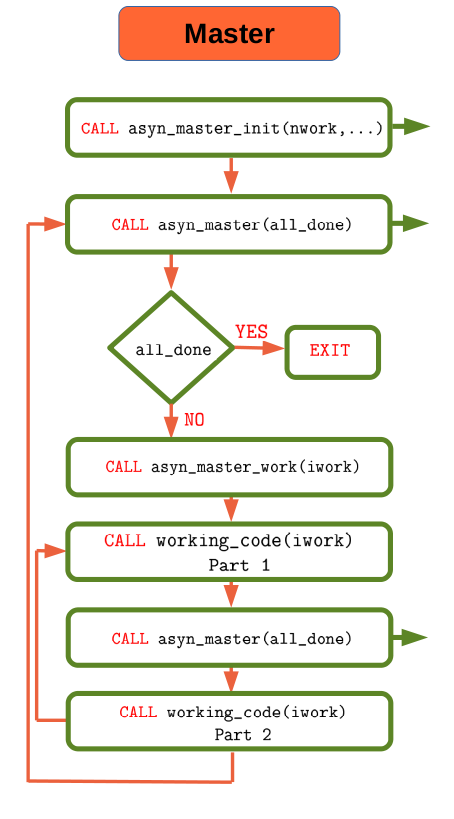
\includegraphics[height=0.80\textwidth]{flowmaster.png}
    &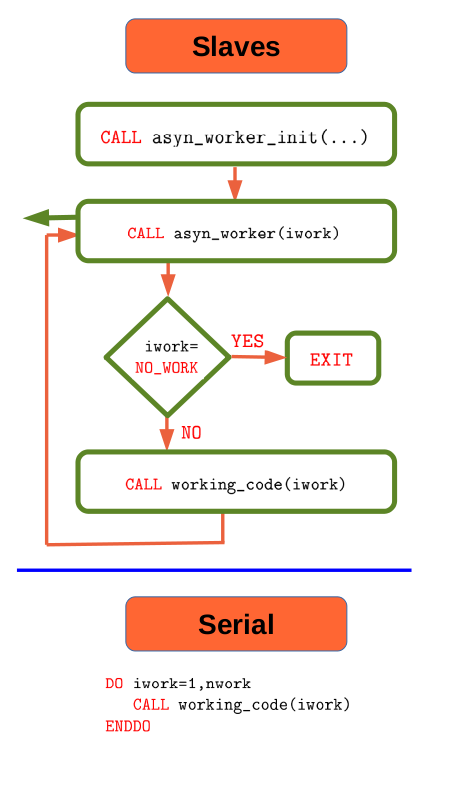
\includegraphics[height=0.80\textwidth]{flowslave.png}\\
  \end{tabular}
 \caption{Comparison between the work-flow of the master image (left)
 and of the slave images (right) in \texttt{thermo\_pw}. In the right
part of the figure we show also the equivalent serial code. The green lines
indicate the points of communication between the master and the slave images.
}
\label{figflow}
\end{figure*}

\end{document}

